\section{Energy loss and gain}\label{sec:3.4}
Until now we have ignored those effects which change the energy of a stored electron; it is now necessary to consider the processes by which an electron loses or gains energy. The lateral acceleration along the curved parts of a trajectory causes an electron to radiate away some of its energy. The characteristics of this radiation loss will be discussed in some detail in Sect. \ref{sec:4.1}. If the electron is to remain captured in the storage ring this radiation loss must be compensated for, on the average, by an equal energy gain from the radio frequency accelerating system of the ring -- one or more electrode structures which produce, along parts of the orbit, an electric field that can feed energy to the moving electron. It is the interplay of the radiation loss and the acceleration gain -- together with the properties of the guide field -- that gathers injected electrons into stable circulating bunches and is responsible for the residual small energy oscillations of the electrons in a bunch.

An electron of the nominal energy $E_0$, moving on the design orbit will radiate away a certain amount of energy, say $U_0$, each revolution. This radiation loss is always a very small fraction (typically $10^{-4}$ or less) of the electron's energy. And the energy gain from the acceleration system is of course, of the same order. The small magnitude of the loss in one revolution allows us, fortunately, to make a number of simplifying assumptions without which a study of the energy oscillations would hardly be tractable. We may, to begin with, make the approximation that an electron which starts a revolution with the energy $E_0$ will also loose the energy $U_0$ during the revolution. Although the energy will not strictly remain at $E_0$, nor the trajectory remain on the design orbit, the deviations during one revolution can be neglected. The effects which accumulate over several revolutions must, however, be taken into account.

If an electron with the energy $E_0$ is given a betatron oscillation its instantaneous rate of radiation loss may change -- because of a different lateral acceleration along the trajectory. But the average energy loss over a complete betatron oscillation will not change to first order in the betatron amplitude. (Changes in the lateral oscillation will be proportional to $x$ and will, to first order, average to zero over a complete
cycle). Since we shall be satisfied to consider only the effects which occur over many betatron oscillations, we need to look only at the average energy loss. So long as we are keeping to our first order view of a storage ring we may ignore any dependence of the radiation loss on the betatron displacements.

The radiation loss will however, change with a change in the energy of an electron. Both its different trajectory and its different energy can contribute to a modified energy loss. Because all energy changes occur slowly, we may consider that an electron is at any instant moving on the off-energy closed orbit which corresponds to its instantaneous energy -- or is performing free betatron oscillations about that orbit. Since we know the form of the off-energy orbit, we can compute the energy lost in each revolution. I shall consider this problem later (in \autoref{sec:4.1}); for now we may take it as a given function $U_{rad}(\epsilon)$ of the energy deviation $\epsilon$.

Since we shall generally be interested only in small energy deviations, we need keep only the linear term in the variation of $U_{rad}$ and write that
\begin{align}
	U_{rad} = U_0 + D\epsilon\label{eq:3.23}
\end{align}
where
\begin{align} \label{eq:3.24}
	D = \left(\frac{dU_{rad}}{d\epsilon}\right)_0
\end{align}
and the derivative is evaluated at the nominal energy $E_0$. For the present, then, the radiation loss may be described by the two constants $U_0$ and $D$ -- which will be evaluated in terms of the properties of the guide field in Chapter \ref{ch:4}.

Let's now turn to the radio frequency accelerating system -- “rf system” for short -- which supplies energy to the electrons to compensate for the radiation loss. The rf system consists typically of one or more cavity resonators such as the one shown schematically in \autoref{fig:fig30}, disposed at various places around the storage ring
and supplied with rf power from some synchronized radio power sources. These cavities produce oscillating electric fields along the electron trajectories; and it is the component of these fields along the electron's path which feeds energy to the electrons. An electron which goes around once on the design orbit will be given by the rf system an amount of energy $U_{rf}$ equal to the integral of the instantaneous electric force along its trajectory.
 
 \begin{figure}[!htb]
 	\centering
 	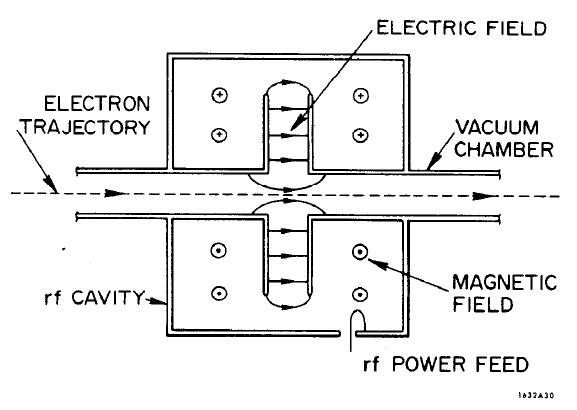
\includegraphics[width=0.7\linewidth]{./Figuras/fig30.jpeg}
 	\caption{Schematic diagram of an rf accelerating cavity.}
 	\label{fig:fig30}
 \end{figure}
 
Since the rf fields are time varying, \footnote{As they must be if there is to be a net integral of the electric field around a closed path!}the energy gained by an electron in making one circuit around the ring will depend on the time at which that circuit begins in relation to the oscillations of the accelerating fields. Let's say that the time dependence of the fields is given. Then the energy $U_{rf}$ gained by the electron -- in one revolution will depend on the time1 that it starts its revolution. (We may take that the revolution starts at some reference azimuth, say $s = 0$.)

If electrons are to be stored on (or near) the design orbit, the variation of $U_{rf}(\bar{t})$ must have certain characteristics. I shall assume that $U_{rf}(\bar{t}$) is a periodic function with a period that is some integral submultiple of the period $T_0$, the period of revolution of an electron that circulates on the design orbit. That is,
\begin{align}
	U_{rf}(\bar{t}+T_0/k) = U_{rf}(\bar{t})\label{eq:3.25}
\end{align}
where $k$ is some integer that will be called the harmonic number of the rf system. The variation of $U_{rf}(\bar{t})$ might be, for example, like the function shown in \autoref{fig:fig31}. (Although the assumed time variation of $U_{rf}$ is somewhat more restrictive than necessary, the rf fields must have at least similar characteristics if a storage ring is to work. And most storage rings will have generally the characteristics assumed.)

\begin{figure}[!htb]
	\centering
	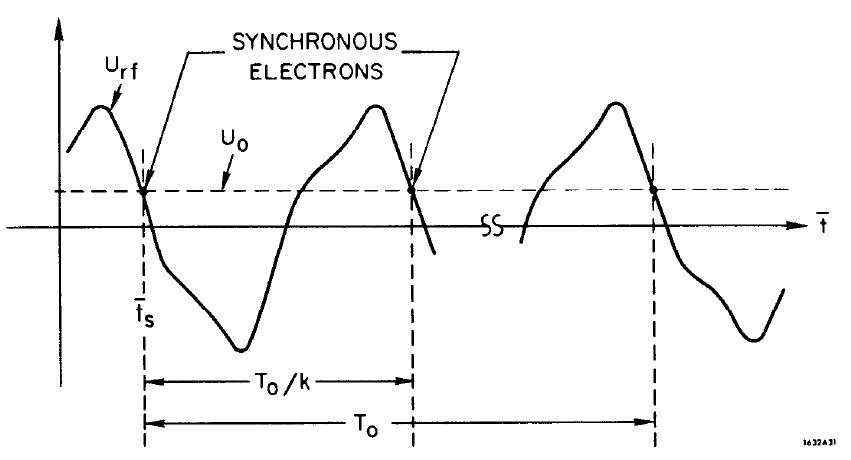
\includegraphics[width=0.85\linewidth]{./Figuras/fig31.jpeg}
	\caption{Energy gain from the rf system as a function of the starting time t of a revolution.}
	\label{fig:fig31}
\end{figure}

Now consider what can happen with an electron of the nominal energy $E_0$ that is circulating on the design orbit. Suppose that it is started on its journey at just the right time $\bar{t}_s$ for which the rf gain $U_{rf}(\bar{t}_s)$ is just equal to the radiation loss $U_0$. See \autoref{fig:fig31}. In the next revolution the energy lost and gained will compensate and the electron will return to its starting point again with the energy $E_0$. The time taken for the revolution is $T_0$; so the electron will start the next revolution at the time $\bar{t}_s + T_0$ and by Eq. \eqref{eq:3.25} the rf gain will again be equal to $U_0$. The electron will continue to circulate indefinitely on the design orbit. Such an electron which passes the reference azimuth at the times $\bar{t}_s + jT_0$ (where $j$ = 1,2,3,..) is called a synchronous electron -- because its rotation is synchronous with the oscillating rf fields. And $\bar{t}_s$ is generally called the synchronous phase of the rf system. (Of course with a periodic rf there are equivalent synchronous starting times once each rf period.)

I have clearly assumed that the peak value of $U_{rf}$ is greater than the radiation loss $U_0$ of the synchronous electron. It follows that there will, in actuality, be
two possible choices (at least) of $\bar{t}_s$ in each cycle of $U_{rf}$ -- one where $U_{rf}$ has a positive slope and one where it has a negative slope. Only one of the two -- the one where the slope is negative -- corresponds to a phase of stable equilibrium, as you will presently see. So only that one will be designated as the synchronous phase $\bar{t}_s$. You can also see from \autoref{fig:fig31} that with a rf harmonic number $k$ there will be $k$ different synchronous starting times -- and therefore, $k$ distinguishable synchronous electrons. These $k$ synchronous phases correspond to $k$ possible stored bunches of electrons.

An electron which is moving with a lateral displacement from the design orbit will see somewhat different electric fields than one moving on the design orbit. It is generally true, however, that its energy gain in one complete revolution -- the path integral of the electric force -- depends very little on the lateral displacements. I shall therefore ignore any dependence of the energy gain on such lateral displacements -- whether they are due to energy deviations or to betatron oscillations -- and consider only the important variation of the energy gain with the starting time $\bar{t}$.

The circulating position of a synchronous electron provides a convenient reference point for the study of the longitudinal oscillations of the electrons in a bunch. We may indeed refer to the moving position of the synchronous electron as the “center” of the bunch and describe the instantaneous azimuthal position of any other electron of the bunch by giving its longitudinal displacement $y$ from the bunch center. That is, we define
\begin{align}
	y(t) = s(t) - s_c(t)
\end{align}
where $s$ is the azimuthal position of any particular electron and $s_c$ refers to the position of the bunch center. See \autoref{fig:fig32}.

\begin{figure}[!htb]
	\centering
	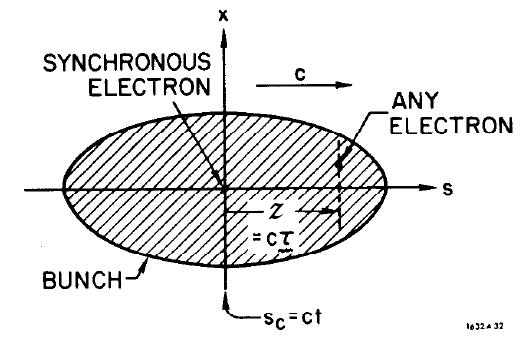
\includegraphics[width=0.6\linewidth]{./Figuras/fig32.jpeg}
	\caption{The longitudinal coordinates $y$ and $\tau$ of an electron in a bunch.}
	\label{fig:fig32}
\end{figure}

For the present discussion I find it somewhat more convenient to describe the longitudinal motion by an equivalent variable $\tau$ defined simply by
\begin{align}
	\tau(t) = y(t)/c
\end{align}
which I shall call the time displacement from the center of the bunch. (The time displacement is very nearly equal to the time interval $\Delta t$ between the arrival of an electron at any particular azimuth and the arrival of the synchronous electron. The difference is equal to the change of $\tau$ in the time $\Delta t = - \tau$ which because of the slow rate of change of $\tau$ can be ignored.) Notice that the time displacement $\tau$ is positive when an electron arrives at each azimuth ahead of the synchronous electron and $\Delta t$ is negative, since it arrives before the synchronous electron.

Because of the time variations of the rf accelerating fields only a synchronous electron will receive the energy $U_0$ each revolution. Any other electron will gain in one revolution an energy $U_{rf}$ which depends on its time displacement $\tau$. We may follow the conventional notation and write
\begin{align}
	U_{rf} = eV(\tau)
\end{align}
where $e$ is the electronic charge and $V(\tau)$ is called the "rf voltagel" -- by analogy with a dc accelerating system. The form of $V(\tau)$ is of course related to $U_{rf}(\tau)$; specifically,
\begin{align}
	eV(\tau) = U_{rf}(\bar{t}_s + \Delta t) = U_{rf}(\bar{t}_s - \tau)
\end{align}
The variation with $\tau$ is reversed from the variation with $\bar{t}$ so the energy gain function of \autoref{fig:fig31} would give the $V(\tau)$ shown in \autoref{fig:fig33} -- where now $\tau = 0$ corresponds to the time displacement of a synchronous electron. Notice that the slope of $V(\tau)$ is positive at $\tau = 0$.

\begin{figure}[!htb]
	\centering
	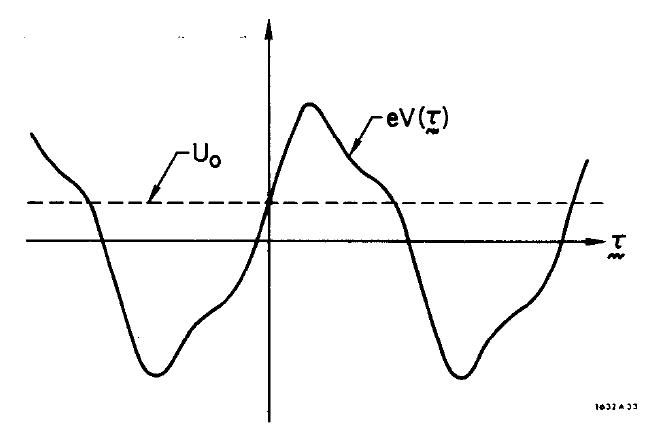
\includegraphics[width=0.6\linewidth]{./Figuras/fig33.jpeg}
	\caption{The rf voltage function $V(\tau)$.}
	\label{fig:fig33}
\end{figure}

It should perhaps be emphasized that the effective "voltage" of a multiple cavity system typical of high energy rings is not simply related to any observable electric "voltage" but depends on the relative positions and oscillation phases of the various rf cavities in the system. The voltage $V(\tau)$ may in fact, depend on the sense of circulation around the ring and may therefore, be quite different for electrons circulating one way around the ring and positrons circulating in the opposite direction.

We are now ready to consider the energy oscillations of an electron in a circulating bunch in a storage ring. Let's first see qualitatively what will happen. Suppose an electron has initially the nominal energy $E_0$ but a positive time displacement $\tau$ -- so that it is ahead of the synchronous position. The radiation loss depends only on the energy so it will be $U_0$ each revolution. But the energy gain will be greater than $U_0$. The electron will gain a little bit of energy each revolution. But an increase in energy will, by Eq. \eqref{eq:3.15}, cause its revolution time to get longer; and its time advance with respect to the bunch center will, accordingly, begin to decrease. After some revolutions the time displacement will decrease to zero. But, by then, the electron's energy will be higher than the nominal energy $E_0$ since the electron has continually been gaining energy -- so the time displacement will continue to decrease now toward negative values of $\tau$. At negative values of $\tau$ however, the energy gain will be too small to compensate for the energy loss by radiation and the electron's energy will begin to decrease toward the nominal energy. When the nominal energy is reached, the time displacement will stop decreasing; but, since it is then negative the energy gain per revolution is below $U_0$ and the energy will begin dropping below $E_0$. Now the time displacement will begin returning toward zero. The process will continue until $\tau$ returns to its starting value, at which point the energy will again be $E_0$.

Let's put this description into quantitative terms. First, take the variation of the time displacement $\tau$. It is convenient to keep track of what is happening by observing a bunch once each revolution when the bunch center is at some arbitrarily chosen reference point. The discussion will be easiest if we take the reference point in some field free region (away from any magnets or rf cavities). In \autoref{fig:fig34} I show two “pictures” of the same bunch on two successive passages of the reference azimuth. In each picture the bunch center is at the reference azimuth so the time between the two pictures is just $T_0$ the revolution time on the design orbit.
 
\begin{figure}[!htb]
	\centering
	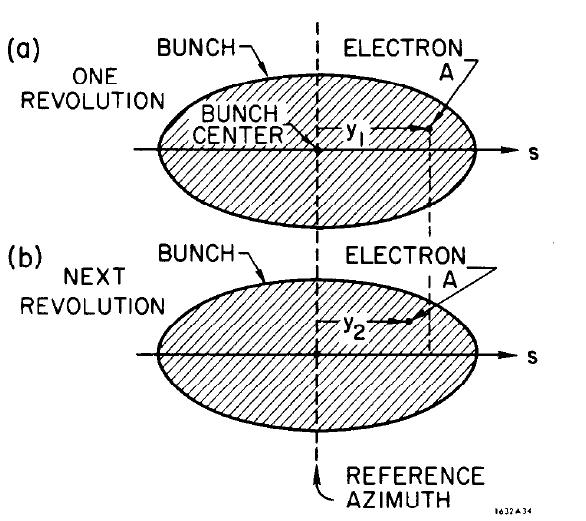
\includegraphics[width=0.6\linewidth]{./Figuras/fig34.jpeg}
	\caption{Longitudinal motion of an electron within a bunch.}
	\label{fig:fig34}
\end{figure}

The pictures show also the position of some particular electron of the bunch: “Electron A”. In the first picture Electron A is ahead of the bunch center by the distance $y_1$. In the second picture the longitudinal displacement has decreased to $y_2$. Between the two pictures the bunch center has traveled once around the design orbit, a distance $L=cT_0$. And since Electron A travels also at the speed $c$, it also has covered a path length equal to $L$. But if it has an energy deviation $\epsilon$ from the nominal energy, the path length for one complete revolution (back to $y_1$) -- would be, as shown in \autoref{sec:3.2}, greater than $L$ by the amount $\delta \ell$ with
\begin{align}
	\frac{\delta \ell}{L} = \alpha\frac{\epsilon}{E_0}
\end{align}
Electron A fails to reach its previous azimuth by the small distance $\delta y = -\delta \ell$, so
\begin{align}
	y_2 - y_1 = \delta y = -\alpha \frac{\epsilon}{E_0}L
\end{align}
The change $\tau$ during the revolution $n$ is
\begin{align}
	\Delta \tau_{n+1} = \frac{\delta y}{c} = -\alpha \frac{\epsilon_n}{E_0}\frac{L}{c} = -\alpha\frac{\epsilon_n}{E_0}T_0
\end{align}
Since the time between the two pictures is $T_0$ the time rate-of-change of $\tau$ is $\Delta \tau/T_0$ or
\begin{align}
	\frac{d \tau}{dt} = -\alpha \frac{\epsilon}{E_0}\label{eq:3.32}
\end{align}
A nice, simple result.

Next, the energy variation. During its revolution Electron A has lost by radiation the energy $U_{rad}(\epsilon)$ and gained from the rf system the energy $eV(\tau)$. The net change in energy during the revolution $n$ is then,
\begin{align}
	\Delta \epsilon_{n+1} = eV(\tau_n)-U_{rad}(\epsilon_n)
\end{align}
The rate-of-change of the energy deviation $\epsilon$ -- when averaged over a complete revolution -- is $\Delta \epsilon/T_0$ so we have that
\begin{align}
	\frac{d\epsilon}{dt} = \frac{eV(\tau)-U_{rad}(\epsilon)}{T_0}\label{eq:3.34}
\end{align}
(We may drop the subscripts on $\tau$ and $\epsilon$ because we may now take it as continuous and derivable variables, since their variation each turn with $T_0$ is sufficiently small, we obtain them by a smooth interpolation from $\tau_1$ to $\tau_2$ to $\tau_3$, etc and $\epsilon_1$ to $\epsilon_2$ to $\epsilon_3$, etc).

The two coupled equations, \eqref{eq:3.32} and \eqref{eq:3.34} describe the energy oscillations -- and the associated oscillations of the time displacement -- of a stored electron. They must be solved together to give the time variation of $\epsilon$ and of $\tau$.

It will turn out -- unfortunately -- that the time displacements which are associated with small energy deviations need not themselves be "small", in the sense that they may span a significant fraction of a complete cycle of the variation of $V(\tau)$. This will be the one instance in which we may not look only at linear terms. We shall need at times to take into account the full nonlinear variations of $V(\tau)$. At other times, however, we shall wish to focus our attention on the small energy oscillations which correspond also to small time displacements. For such oscillations we shall need to retain only the linear part of the variation of $V(\tau)$. Since the acceleration energy gain at $\tau = 0$ is by definition $U_0$, we may then write
\begin{align}
	U_{rf} = eV(\tau) = U_0 + e\dot{V}_0\tau\label{eq:3.35}
\end{align}
where $\dot{V}_0$ stands for $dV/d\tau$ evaluated at $\tau=0$.

It is quite common for the rf voltage of a storage ring to have a sinusoidal variation with time. In such cases we would have that
\begin{align}\label{eq:3.36}
	V(\tau) = \widehat{V} \sin(\omega_{rf}(\tau+\tau_0))
\end{align}
where $\widehat{V}$ is called the “peak rf voltage" and $\omega_{rf}\tau_0$  is called the "synchronous rf phase angle". With our assumptions
\begin{align}
	\omega_{rf} = 2\pi \frac{k}{T_0} = k\omega_r
\end{align}
It also follows that
\begin{align}
	\omega_{rf}\tau_0 = \arcsin(U_0/e\widehat{V})
\end{align}
and that
\begin{align}
	\dot{V}_0 = \omega_{rf}\widehat{V}cos(\omega_{rf}\tau_0) = \omega_{rf}\widehat{V}\left[1-\left(\frac{U_0}{e\widehat{V}}\right)^2\right]^{1/2}
\end{align}
